\batchmode
\makeatletter
\def\input@path{{./}{_dependencies/}}
\makeatother
\documentclass[english,notheorems]{beamer}\usepackage[]{graphicx}\usepackage[]{xcolor}
\makeatletter
\def\maxwidth{   \ifdim\Gin@nat@width>\linewidth
    \linewidth
  \else
    \Gin@nat@width
  \fi
}
\makeatother

\definecolor{fgcolor}{rgb}{0.345, 0.345, 0.345}
\newcommand{\hlnum}[1]{\textcolor[rgb]{0.686,0.059,0.569}{#1}}\newcommand{\hlsng}[1]{\textcolor[rgb]{0.192,0.494,0.8}{#1}}\newcommand{\hlcom}[1]{\textcolor[rgb]{0.678,0.584,0.686}{\textit{#1}}}\newcommand{\hlopt}[1]{\textcolor[rgb]{0,0,0}{#1}}\newcommand{\hldef}[1]{\textcolor[rgb]{0.345,0.345,0.345}{#1}}\newcommand{\hlkwa}[1]{\textcolor[rgb]{0.161,0.373,0.58}{\textbf{#1}}}\newcommand{\hlkwb}[1]{\textcolor[rgb]{0.69,0.353,0.396}{#1}}\newcommand{\hlkwc}[1]{\textcolor[rgb]{0.333,0.667,0.333}{#1}}\newcommand{\hlkwd}[1]{\textcolor[rgb]{0.737,0.353,0.396}{\textbf{#1}}}\let\hlipl\hlkwb

\usepackage{framed}
\makeatletter
\newenvironment{kframe}{ \def\at@end@of@kframe{} \ifinner\ifhmode  \def\at@end@of@kframe{\end{minipage}}  \begin{minipage}{\columnwidth} \fi\fi \def\FrameCommand##1{\hskip\@totalleftmargin \hskip-\fboxsep
 \colorbox{shadecolor}{##1}\hskip-\fboxsep
          \hskip-\linewidth \hskip-\@totalleftmargin \hskip\columnwidth} \MakeFramed {\advance\hsize-\width
   \@totalleftmargin\z@ \linewidth\hsize
   \@setminipage}} {\par\unskip\endMakeFramed \at@end@of@kframe}
\makeatother

\definecolor{shadecolor}{rgb}{.97, .97, .97}
\definecolor{messagecolor}{rgb}{0, 0, 0}
\definecolor{warningcolor}{rgb}{1, 0, 1}
\definecolor{errorcolor}{rgb}{1, 0, 0}
\newenvironment{knitrout}{}{} 
\usepackage{alltt}
\PassOptionsToPackage{natbib=true}{biblatex}
\usepackage[T1]{fontenc}
\usepackage[utf8]{inputenc}
\setcounter{secnumdepth}{4}
\setcounter{tocdepth}{3}
\usepackage{mathtools}
\usepackage{amstext}
\usepackage{amsthm}
\usepackage{amssymb}
\usepackage{xargs}[2008/03/08]
\PassOptionsToPackage{normalem}{ulem}
\usepackage{ulem}

\makeatletter
\newcommand\makebeamertitle{\frame{\maketitle}}\AtBeginDocument{  \let\origtableofcontents=\tableofcontents
  \def\tableofcontents{\@ifnextchar[{\origtableofcontents}{\gobbletableofcontents}}
  \def\gobbletableofcontents#1{\origtableofcontents}
}

\setbeamerfont{frametitle}{size=\fontsize{15}{18}\selectfont}

\setbeamertemplate{navigation symbols}{}

  \setbeamertemplate{footline}[frame number]{}

\setbeamertemplate{section in toc}{\inserttocsectionnumber.~\inserttocsection}

\setbeamercolor{alerted text}{fg=blue}

\setbeamertemplate{theorems}[numbered]

\setbeamertemplate{note page}[plain]

\addtobeamertemplate{block begin}{\vskip -\bigskipamount}{}
\addtobeamertemplate{block end}{}{\vskip -\smallskipamount}
\addtobeamertemplate{block alerted begin}{\vskip -\bigskipamount}{}
\addtobeamertemplate{block alerted begin}{}{\vskip -\smallskipamount}


\newcommand*\Alt{\alt{\Alt@branch0}{\Alt@branch1}}

\newcommand\Alt@branch[3]{  \begingroup
  \ifbool{mmode}{    \mathchoice{      \Alt@math#1{\displaystyle}{#2}{#3}    }{      \Alt@math#1{\textstyle}{#2}{#3}    }{      \Alt@math#1{\scriptstyle}{#2}{#3}    }{      \Alt@math#1{\scriptscriptstyle}{#2}{#3}    }  }{    \sbox0{#2}    \sbox1{#3}    \Alt@typeset#1  }  \endgroup
}

\newcommand\Alt@math[4]{  \sbox0{$#2{#3}\m@th$}  \sbox1{$#2{#4}\m@th$}  \Alt@typeset#1}

\newcommand\Alt@typeset[1]{  \ifnumcomp{\wd0}{>}{\wd1}{    \def\setwider   ##1##2{##2##1##2 0}    \def\setnarrower##1##2{##2##1##2 1}  }{    \def\setwider   ##1##2{##2##1##2 1}    \def\setnarrower##1##2{##2##1##2 0}  }  \sbox2{}  \sbox3{}  \setwider2{\wd}  \setwider2{\ht}  \setwider2{\dp}  \setnarrower3{\ht}  \setnarrower3{\dp}  \leavevmode
  \rlap{\usebox#1}  \usebox2  \usebox3}

\newcommand{\altQ}[1]{\alert<.(1)|handout:0>{\alt<+->{#1}{\omcolorA{?}}}}
\newcommand{\AltQ}[1]{\alert<.(1)|handout:0>{\Alt<+->{#1}{\omcolorA{?}}}}
\newcommand{\smallrelstack}{\mathrel{  \smash{    \vcenter{\hbox{      \scalebox{0.4}{$
        \begin{array}{c}
          ?\\[-0.35em]
          <\\[-0.35em]
          >\\[-0.35em]
          =
        \end{array}
      $}    }}  }}}
\newcommand{\relQ}[1]{\mathrel{  \alert<.(1)|handout:0>{    \Alt<+->{#1}{\omcolorA{\smallrelstack}}  }}}

\newcommand{\stackSmallerOrLarger}{\mathrel{  \smash{    \vcenter{\hbox{      \scalebox{0.4}{$
        \begin{array}{c}
          ?\\[-0.35em]
          \text{smaller}\\[-0.35em]
          \text{larger}
        \end{array}
      $}    }}  }}}
\newcommand{\smallerOrLarger}[1]{\mathrel{  \alert<.(1)|handout:0>{    \Alt<+->{#1}{\omcolorA{\stackSmallerOrLarger}}  }}}


\usepackage{amsbsy}
\usepackage{stackrel}

\newcommand{\omDistributedUnderNull}{\underset{\smash{\raisebox{0.7ex}{\scalebox{0.45}{$H_0$}}}}{\sim}}
\newcommand{\omApproximatelyDistributedUnderNull}{\stackrel[{\smash{\raisebox{0.7ex}{\scalebox{0.45}{$H_0$}}}}]{\boldsymbol{\cdot}}{\sim}
}

\newcommand{\dotsUncover}[1]{\alert<.(1)|handout:0>{\only<.|handout:0>{\rlap{\ldots}}\uncover<+->{#1}}}

\newcommand{\dotsUncoverQ}[1]{\alert<.(1)|handout:0>{\only<.|handout:0>{\rlap{\ldots?}}\uncover<+->{#1}}}

\newcommand{\altAlert}[2]{\alert<.(1)|handout:0>{\alt<+->{#2}{#1}}}


\usepackage{scalerel}

\makeatletter
\newlength{\gapwidth}
\newlength{\gapheight}
\newlength{\gapdepth}
\newbox\blankQ@measurebox
\newif\ifblankQ@underline

\newcommand{\blankQ}[2][]{\begingroup\blankQ@underlinetrue\def\blankQ@option{#1}\def\blankQ@nounderline{nounderline}\ifx\blankQ@option\blankQ@nounderline
  \blankQ@underlinefalse\fi
\edef\beamerpauses@backup{\arabic{beamerpauses}}\ThisStyle{  \ifmmode
    \setbox\blankQ@measurebox=\hbox{$\SavedStyle#2$}  \else
    \setbox\blankQ@measurebox=\hbox{#2}  \fi
  \gapwidth=\wd\blankQ@measurebox
  \gapheight=\ht\blankQ@measurebox
  \gapdepth=\dp\blankQ@measurebox
  \setcounter{beamerpauses}{\beamerpauses@backup}  \alert<.(1)|handout:0>{    \alt<+->{      #2    }{      \rule[-\gapdepth]{0pt}{\dimexpr\gapheight+\gapdepth\relax}      \omcolorA{        \smash{          \ifmmode
            \ifblankQ@underline
              \underline{\makebox[\gapwidth]{$\SavedStyle ?$}}            \else
              \makebox[\gapwidth]{$\SavedStyle ?$}            \fi
          \else
            \ifblankQ@underline
              \underline{\makebox[\gapwidth]{?}}            \else
              \makebox[\gapwidth]{?}            \fi
          \fi
        }      }    }  }}\endgroup}
\makeatother





\providecommand{\omsubtitle}{
}

\setbeamertemplate{enumerate subitem}{\alph{enumii}.}
\setbeamertemplate{itemize subitem}[circle]
\setbeamertemplate{itemize subsubitem}[square]

\AtBeginEnvironment{align}{\setcounter{equation}{0}}

\setbeamertemplate{theorem begin}
{\begin{\inserttheoremblockenv}
  {}{\usebeamerfont*{block title}\usebeamercolor[fg]{block title}          \inserttheoremname
  \inserttheoremnumber
  \ifx \inserttheoremaddition \empty \else\ (\inserttheoremaddition)\fi
  \inserttheorempunctuation}
  \normalfont
  }
  \setbeamertemplate{theorem end}{\end{\inserttheoremblockenv}}

\newcommand{\ombasecolorA}{teal}

\newcommand{\omalertA}{\detokenize{alert@+|+-}}
\newcommand{\omalertAat}{\detokenize{alert@}}
\newcommand{\omalertB}{\detokenize{alert@+|+-}}

\beamerdefaultoverlayspecification{<\omalertA>}

\makeatletter
\DeclareRobustCommand*{\savepause}[2][0]{\only<1>{  \immediate\write\@auxout{\string\pauseentry
  {\the\c@framenumber}{#2}{\number\numexpr\c@beamerpauses-#1\relax}}}}

\newcommand*{\usepause}[1]{\@ifundefined{pauses@  \the\c@framenumber @#1}{1}{\@nameuse{pauses@\the\c@framenumber @#1}}}

\def\usepauseoffset[#1]#2{\number\numexpr\usepause{#2}+#1\relax}

\newcommand*{\pauseentry}[3]{\global\@namedef{pauses@#1@#2}{#3}}
\makeatother

\setbeamercolor{frametitle}{fg=black}

\usepackage{array}

\usepackage{colortbl}

\mode<handout>{
  \setbeamercolor{alerted text}{fg=black}
}

\newcommand{\omcolorA}[1]{\textcolor{\ombasecolorA} {#1}}
\newcommand{\omcolorB}[1]{\textcolor{purple} {#1}}
\newcommand{\omcolorC}[1]{\textcolor{brown} {#1}}

\newcommand{\omcolorPreserveMath}[2]{\begingroup
\color{#1}#2\endgroup
}

\newcommand*\RrvealGroupColorsList{\ombasecolorA}

\makeatletter
\newcommand*\newreveal{\@newl@bel{revealgroup}}

\newcommand*\NewRevealGroup[3]{  \expandafter\newcommand\csname revealGroup#3\endcsname[1]{      \only<.>{          \immediate\write\@auxout{              \string\newreveal{Group#3-Frame\theframenumber}{\the\beamer@slideinframe}          }      }      \alt<.|handout:0>{          \omcolorPreserveMath{#2}{##1}      }{          ##1      }  }  
    \expandafter\newcommand\csname groupAon#3\endcsname[1]{      \@ifundefined{revealgroup@Group#3-Frame\theframenumber}{          ##1      }{          \alt<\csname revealgroup@Group#3-Frame\theframenumber\endcsname|handout:0>{              \omcolorPreserveMath{\ombasecolorA}{##1}          }{              ##1          }      }  }
  \expandafter\newcommand\csname groupBon#3\endcsname[1]{      \@ifundefined{revealgroup@Group#3-Frame\theframenumber}{          ##1      }{          \alt<\csname revealgroup@Group#3-Frame\theframenumber\endcsname|handout:0>{              \omcolorPreserveMath{purple}{##1}          }{              ##1          }      }  }
  \expandafter\newcommand\csname groupCon#3\endcsname[1]{      \@ifundefined{revealgroup@Group#3-Frame\theframenumber}{          ##1      }{          \alt<\csname revealgroup@Group#3-Frame\theframenumber\endcsname|handout:0>{              \omcolorPreserveMath{brown}{##1}          }{              ##1          }      }  }
  \expandafter\newcommand\csname qBefore#3\endcsname[1]{            \@ifundefined{revealgroup@Group#3-Frame\theframenumber}{          ##1      }{          \Alt<\csname revealgroup@Group#3-Frame\theframenumber\endcsname ->{##1}{?}      }  }
      \expandafter\newcommand\csname AltOn#3\endcsname[2]{            \@ifundefined{revealgroup@Group#3-Frame\theframenumber}{          ##1      }{          \Alt<\csname revealgroup@Group#3-Frame\theframenumber\endcsname ->{##1}{##2}      }  }}

\newcounter{RevealGroup}
\@for\group@color:=\RrvealGroupColorsList\do{  \stepcounter{RevealGroup}  \@expandtwoargs\NewRevealGroup{\Alph{RevealGroup}}{\group@color}{One}  \@expandtwoargs\NewRevealGroup{\Alph{RevealGroup}}{purple}{Two}  \@expandtwoargs\NewRevealGroup{\Alph{RevealGroup}}{brown}{Three}  \@expandtwoargs\NewRevealGroup{\Alph{RevealGroup}}{yellow}{Four}  \@expandtwoargs\NewRevealGroup{\Alph{RevealGroup}}{pink}{Five}  \@expandtwoargs\NewRevealGroup{\Alph{RevealGroup}}{blue}{Six}  \@expandtwoargs\NewRevealGroup{\Alph{RevealGroup}}{black}{Seven}  \@expandtwoargs\NewRevealGroup{\Alph{RevealGroup}}{orange}{Eight}}
\makeatother

\newcommand{\colorAonOne}[1]{\groupAonOne{#1}}\newcommand{\colorBonOne}[1]{\groupBonOne{#1}}\newcommand{\colorConOne}[1]{\groupConOne{#1}}\newcommand{\colorAonTwo}[1]{\groupAonTwo{#1}}\newcommand{\colorBonTwo}[1]{\groupBonTwo{#1}}\newcommand{\colorConTwo}[1]{\groupConTwo{#1}}\newcommand{\colorAonThree}[1]{\groupAonThree{#1}}\newcommand{\colorBonThree}[1]{\groupBonThree{#1}}\newcommand{\colorConThree}[1]{\groupConThree{#1}}\newcommand{\colorAonFour}[1]{\groupAonFour{#1}}\newcommand{\colorBonFour}[1]{\groupBonFour{#1}}\newcommand{\colorConFour}[1]{\groupConFour{#1}}\newcommand{\colorAonFive}[1]{\groupAonFive{#1}}\newcommand{\colorBonFive}[1]{\groupBonFive{#1}}\newcommand{\colorConFive}[1]{\groupConFive{#1}}\newcommand{\colorAonSix}[1]{\groupAonSix{#1}}\newcommand{\colorBonSix}[1]{\groupBonSix{#1}}\newcommand{\colorConSix}[1]{\groupConSix{#1}}\newcommand{\colorAonSeven}[1]{\groupAonSeven{#1}}\newcommand{\colorBonSeven}[1]{\groupBonSeven{#1}}\newcommand{\colorConSeven}[1]{\groupConSeven{#1}}\newcommand{\colorAonEight}[1]{\groupAonEight{#1}}\newcommand{\colorBonEight}[1]{\groupBonEight{#1}}\newcommand{\colorConEight}[1]{\groupConEight{#1}}\newcommand{\triggerOne}[1]{\revealGroupOne{#1}}\newcommand{\triggerTwo}[1]{\revealGroupTwo{#1}}\newcommand{\triggerThree}[1]{\revealGroupThree{#1}}\newcommand{\triggerFour}[1]{\revealGroupFour{#1}}\newcommand{\triggerFive}[1]{\revealGroupFive{#1}}\newcommand{\triggerSix}[1]{\revealGroupSix{#1}}\newcommand{\triggerSeven}[1]{\revealGroupSeven{#1}}\newcommand{\triggerEight}[1]{\revealGroupEight{#1}}

\usepackage{stackengine,scalerel}
\let\oldPhi\Phi
\newcommand\altPhi{\ThisStyle{\ensurestackMath{
\stackengine{-.6\LMpt}{\stackengine{-.7\LMpt}{\SavedStyle\oldPhi}{\rule{.5\LMex}{.7\LMpt}\kern.01ex}
  {U}{c}{F}{F}{S}}{\rule{.5\LMex}{.7\LMpt}\kern.01ex}{O}{c}{F}{F}{S}}}}
\let\Phi\altPhi

\makeatletter
\newcommand*{\cleq}[1][green]{\mathrel{\mathpalette\c@leq{#1}}}
\newcommand*{\c@leq}[2]{ \m@th
 \setbox\z@\hbox{{\color{#2}$#1-$}} \dp\z@\z@
 \vcenter{\offinterlineskip\ialign{##\cr$#1<$\cr\noalign{\kern-.3\ht\z@}\copy\z@\cr\noalign{\kern-.45\ht\z@}}}}
\makeatother


\newcommand{\omFinalAnswer}[1]{\textcolor<.>{orange} {#1}}

\usepackage[misc]{ifsym}
\usepackage{tikz}
\usepackage{pgfplots}
\pgfplotsset{compat=1.18}
\newcommand{\tcancel}[2][thick]{\begin{tikzpicture}
\node[inner sep=1pt] (a){#2};
\draw[#1] (a.south west) -- (a.north east);
\draw[#1] (a.north west) -- (a.south east);
\end{tikzpicture}}

\usepackage{twemojis}
\newcommand{\mousetrap}{\twemoji{mouse trap}}








\makeatletter
\ExplSyntaxOn
\bool_new:N \l__bseq_noparens_bool
\bool_new:N \l__bseq_fill_bool
\keys_define:nn { bseq } {
noparens .bool_set:N = \l__bseq_noparens_bool,
fill     .bool_set:N = \l__bseq_fill_bool,
}
\cs_new_protected:Npn \bseq_parse:n #1 {
\bool_set_false:N \l__bseq_noparens_bool
\bool_set_false:N \l__bseq_fill_bool
\keys_set:nn { bseq } { #1 }
}

\newcount\bseq@currentid
\newcount\bseq@position
\bseq@currentid=0
\bseq@position=0

\def\bseq@settotal#1#2{\expandafter\gdef\csname bseq@total@#1\endcsname{#2}}
\def\bseq@gettotal#1{\@ifundefined{bseq@total@#1}{??}{\csname bseq@total@#1\endcsname}}
\def\bseq@writepos{\immediate\write\@auxout{\string\bseq@settotal{\the\bseq@currentid}{\the\bseq@position}}}
\def\bseq@remember{\expandafter\xdef\csname bseq@frameid@\the\c@framenumber\endcsname{\the\bseq@currentid}\expandafter\xdef\csname bseq@framepos@\the\c@framenumber\endcsname{\the\bseq@position}}
\def\bseq@print{\expandafter\let\expandafter\bseq@printid\csname bseq@frameid@\the\c@framenumber\endcsname
\csname bseq@name@\bseq@printid\endcsname
\ifnum\csname bseq@fill@\bseq@printid\endcsname=1\relax \hfill\else\space\fi
\ifnum\csname bseq@parens@\bseq@printid\endcsname=1\relax
   (\csname bseq@framepos@\the\c@framenumber\endcsname/\bseq@gettotal{\bseq@printid})\else
   \csname bseq@framepos@\the\c@framenumber\endcsname/\bseq@gettotal{\bseq@printid}\fi
}

\NewDocumentCommand\startTitleSeq{ O{} m }{\@ifundefined{bseq@frameid@\the\c@framenumber}{  \bseq_parse:n{#1}    \global\bseq@currentid=\c@framenumber\relax
  \global\bseq@position=1\relax
  \expandafter\gdef\csname bseq@name@\the\bseq@currentid\endcsname{#2}  \bool_if:NTF \l__bseq_noparens_bool
    {\expandafter\gdef\csname bseq@parens@\the\bseq@currentid\endcsname{0}}
    {\expandafter\gdef\csname bseq@parens@\the\bseq@currentid\endcsname{1}}  \bool_if:NTF \l__bseq_fill_bool
    {\expandafter\gdef\csname bseq@fill@\the\bseq@currentid\endcsname{1}}
    {\expandafter\gdef\csname bseq@fill@\the\bseq@currentid\endcsname{0}}  \bseq@remember
  \bseq@writepos
}{}\bseq@print
}
\NewDocumentCommand\continueTitleSeq{}{\@ifundefined{bseq@frameid@\the\c@framenumber}{  \ifnum\bseq@currentid=0\relax
    \PackageError{bseq}{\string\continueTitleSeq\space before \string\startTitleSeq}{}  \else
    \global\advance\bseq@position by 1\relax
    \bseq@remember
    \bseq@writepos
  \fi
}{}\ifnum\bseq@currentid>0\relax \bseq@print\fi
}
\NewDocumentCommand\stepTitleSeqNum{}{\@ifundefined{bseq@stepped@\the\c@framenumber}{  \ifnum\bseq@currentid=0\relax
    \PackageError{bseq}{\string\stepTitleSeqNum\space before \string\startTitleSeq}{}  \else
    \global\advance\bseq@position by 1\relax
    \expandafter\gdef\csname bseq@stepped@\the\c@framenumber\endcsname{1}    \bseq@writepos
  \fi
}{}}
\ExplSyntaxOff
\makeatother

\newcommand{\extractThisLabelForReview}[1]{}

\newcommand{\hypertargetprevpause}[2]{\begingroup
\edef\x{\endgroup
  \noexpand\hypertarget<\number\numexpr\value{beamerpauses}-1\relax>{#1}{#2}}\x
}


\newcommand{\omeqcolor}[1]{\begingroup
\color{green}#1\endgroup
}
\newcommand{\omeqcolorB}[1]{\begingroup
\color{purple}#1\endgroup
}
\newcommand{\omeqcolorC}[1]{\begingroup
\color{brown}#1\endgroup
}

\AtEndEnvironment{knitrout}{\vspace{-0.5\baselineskip plus 0.5\baselineskip minus 0.5\baselineskip}}



\AtBeginDocument{\setlength{\abovedisplayskip}{6pt plus 10pt minus 10pt}\setlength{\belowdisplayskip}{6pt plus 10pt minus 10pt}\setlength{\abovedisplayshortskip}{2pt plus 4pt minus 2pt}\setlength{\belowdisplayshortskip}{2pt plus 4pt minus 2pt}}






\makeatletter

\useoutertheme[subsection=false]{miniframes}

\setbeamertemplate{headline}{\begin{beamercolorbox}[wd=\paperwidth,ht=2.2ex,dp=0.9ex]{palette tertiary}  \insertnavigation{\paperwidth}\end{beamercolorbox}}
\newsavebox{\frametitlemeasurebox}
\setbeamertemplate{frametitle}{\nointerlineskip
\begin{beamercolorbox}[wd=\paperwidth,ht=2.3ex,dp=0.8ex,leftskip=0.3cm,rightskip=0.3cm]{frametitle}  \usebeamerfont{frametitle}  \sbox{\frametitlemeasurebox}{\insertframetitle}  \ifdim\wd\frametitlemeasurebox>\dimexpr\paperwidth-0.6cm\relax
    \PackageError{beamer}      {Frame title too wide: \detokenize\expandafter{\insertframetitle}}      {Shorten the frame title.}  \fi
  \insertframetitle
\end{beamercolorbox}}

\usepackage{xparse}

\let\origsection\section
\let\origsubsection\subsection

\RenewDocumentCommand{\section}{som}{  }


\RenewDocumentCommand{\subsection}{som}{  \IfBooleanTF{#1}{                        \section*{#3}  }{    \IfNoValueTF{#2}
      {\origsection{#3}}      {\origsection[#2]{#3}}  }}

\usepackage{etoolbox}
\makeatletter
\patchcmd{\slideentry}{\advance\beamer@tempdim by -.05cm}{\advance\beamer@tempdim by\beamer@vboxoffset\advance\beamer@tempdim by\beamer@boxsize\advance\beamer@tempdim by 1.2\pgflinewidth}{}{}
\patchcmd{\slideentry}{\kern\beamer@tempdim}{\advance\beamer@tempdim by 2pt\advance\beamer@tempdim by\wd\beamer@sectionbox\kern\beamer@tempdim}{}{}
\patchcmd\beamer@@tmpl@button{\pgfsetlinewidth{0.8pt}}{}{}{}
\setbeamertemplate{mini frame}{\beamer@xelatex@fixminiframes
\ifnum\insertframeendpage=\thepage
  \mode<presentation>{                \color{gray}  }      \mode<handout>{    \color{black}  }\fi
\begin{pgfpicture}{0pt}{0pt}{0.1cm}{0.1cm}
  \pgfpathcircle{\pgfpoint{0.05cm}{0.05cm}}{0.05cm}
  \pgfusepath{fill,stroke}
\end{pgfpicture}}
\makeatother


\makeatletter
\let\beamer@writeslidentry@miniframeson=\beamer@writeslidentry
\def\beamer@writeslidentry@miniframesoff{\expandafter\beamer@ifempty\expandafter{\beamer@framestartpage}{}{  \clearpage\beamer@notesactions}}
\newcommand*{\miniframeson}{\let\beamer@writeslidentry=\beamer@writeslidentry@miniframeson}
\newcommand*{\miniframesoff}{\let\beamer@writeslidentry=\beamer@writeslidentry@miniframesoff}


\usepackage{etoolbox}

\newsavebox\onblackboardbox    \newcounter{omx}        \resetcounteronoverlays{omx}                        \newenvironment{omx}[1][]    {            \refstepcounter{omx}
                \list{}{    \leftmargin=0em                    \topsep=1.75ex plus 1.75ex minus 1.75ex    \parsep=\parskip    \listparindent=\parindent    \itemindent=\parindent  }\item\relax    \begin{lrbox}{\onblackboardbox}      \begin{minipage}{\hsize}      \begin{uncoverenv}<+->            \begin{alertenv}<.|handout:0>                  \ifstrempty{#1} {                        \textbf{\structure{Exercise~\theomx}}.       } {        \textbf{\structure{Exercise~\theomx~(#1)}}.       }    }    {     \end{alertenv}     \end{uncoverenv}     \end{minipage}    \end{lrbox}            \mode<handout>{\usebox{\onblackboardbox}}        \mode<beamer|second|trans|article>{\usebox{\onblackboardbox}}    \endlist  }
\newsavebox\presbox\newcommand{\onlypres}[1]{\relax \begin{lrbox}{\presbox}   \begin{minipage}{\hsize}   #1     \end{minipage}    \end{lrbox}            \mode<handout>{\usebox{\presbox}}
        \mode<beamer|second|trans|article>{\usebox{\presbox}}}
\ExplSyntaxOn
\makeatother

\cs_new_eq:NN \_overlayalign_orig_align: \align
\cs_new_eq:NN \end_overlayalign_orig_align: \endalign

\cs_new_eq:Nc \_overlayalign_orig_starred_align: { align* }
\cs_new_eq:NN \end_overlayalign_orig_starred_align: \endalign

\seq_new:N \l__overlayalign_linesin_seq
\seq_new:N \l__overlayalign_linesout_seq
\seq_new:N \l__overlayalign_onelinein_seq
\seq_new:N \l__overlayalign_onelineout_seq
\int_new:N \g_overlayalign_currpause_int

\cs_new:Npn \overlayalign_add_alert_to_cells:n #1
  {
    \seq_set_split:Nnn \l__overlayalign_linesin_seq { \\ } { #1 }
    \seq_map_inline:Nn \l__overlayalign_linesin_seq
    {
        \seq_clear:N \l__overlayalign_onelineout_seq
        \seq_set_split:Nnn \l__overlayalign_onelinein_seq { & } { ##1 }
        \seq_map_indexed_inline:Nn \l__overlayalign_onelinein_seq
        {
            \int_compare:nNnTF { ####1 } = { 1 }
            {
              \seq_put_right:Nn \l__overlayalign_onelineout_seq {
                \action<+-|alert@+> {
                  \int_gset:Nn \g_overlayalign_currpause_int { \value{beamerpauses} - 1 }
                  ####2
                }
              }
            }
            {
              \seq_put_right:Nn \l__overlayalign_onelineout_seq {
                \action<\g_overlayalign_currpause_int-|alert@\g_overlayalign_currpause_int> { ####2 } }
            }
        }
        \seq_put_right:Ne \l__overlayalign_linesout_seq { \seq_use:Nn \l__overlayalign_onelineout_seq { & } }
    }
  }

\newenvironment{overlayalign}{
    \RenewDocumentEnvironment{align}{+b}
    {
        \cs_set_nopar:cpn { tagform@ } ####1
            {
                \use:c { maketag@@@ }
                  {
                    \action<\g_overlayalign_currpause_int-|alert@\g_overlayalign_currpause_int>
                      { ( \ignorespaces ####1 \unskip \use:c { @@italiccorr } ) }
                  }
            }
        \overlayalign_add_alert_to_cells:n { ##1 }
        \begin{_overlayalign_orig_align:}
            \seq_use:Nn \l__overlayalign_linesout_seq { \\ }
        \end{_overlayalign_orig_align:}
    } { }
    \RenewDocumentEnvironment{align*}{+b}
    {
        \overlayalign_add_alert_to_cells:n { ##1 }
        \begin{_overlayalign_orig_starred_align:}
            \seq_use:Nn \l__overlayalign_linesout_seq { \\ }
        \end{_overlayalign_orig_starred_align:}
    } { }
}{ }
\makeatletter
\ExplSyntaxOff
\newcommand{\omemphA}[1]{\emph {#1}}
\newcommand{\answer}[1]{\rule[0.5ex]{1\columnwidth}{1pt}\par\nobreak A: #1}

\makeatother

\providecommand\definitionname{Definition}
\theoremstyle{definition}
\newtheorem{defn}{\protect\definitionname}
\providecommand\theoremname{Theorem}
\theoremstyle{plain}
\newtheorem{thm}{\protect\theoremname}
\providecommand\notationname{Notation}
\theoremstyle{remark}
\newtheorem{notation}{\protect\notationname}
\usepackage{babel}
\usepackage[style=authoryear,maxcitenames=4]{biblatex}
\usepackage{environ}
  	\providecommand{\omxname}{OMX}

\usepackage{etoolbox}
\IfFileExists{upquote.sty}{\usepackage{upquote}}{}
\begin{document}
\title{Expected value and variance}
\institute{\omsubtitle}

\makebeamertitle
\global\long\def\omPr{\mathrm{P}}
\global\long\def\omE{\mathrm{E}}
\global\long\def\omV{\mathrm{V}}
\global\long\def\omSD{\mathrm{SD}}
\global\long\def\omSE{\mathrm{SE}}
\global\long\def\omCov{\mathrm{cov}}
\global\long\def\omCorr{\mathrm{corr}}
\global\long\def\argmin{\mathrm{argmin}}
\global\long\def\omSupp#1{\mathrm{supp}(#1)}
\global\long\def\omIndicatorFunction{\mathrm{I}}
\global\long\def\omError{\mathrm{u}}
\global\long\def\omOLS#1{#1^{OLS}}




\global\long\def\eqq{\overset{\smash{?}}{=}}
\def\independenT#1#2{\mathrel{\rlap{$#1#2$}\mkern5mu{#1#2}}}

\global\long\def\independent#1#2{#1\mathpalette{\independenT}{\perp}#2}
\global\long\def\notIndependent#1#2{#1\not\mathpalette{\independenT}{\perp}#2}
\global\long\def\rvDieEven{T}
\global\long\def\rvDieNum{D}
\global\long\def\obsDieNum{d}
\global\long\def\rvNumHeads{Y}
\global\long\def\rvNumTails{Z}
\global\long\def\rvHearts{H}
\global\long\def\rvQuarter{Q}
\global\long\def\rvIncome{X}
\global\long\def\obsIncome{x}
\global\long\def\nIncome{5}
\global\long\def\ombar#1{\bar{#1}}
\global\long\def\omerror{u}
\global\long\def\omcoloneqq{\coloneqq}
\ExplSyntaxOn
\ProvideDocumentCommand \xilistprivate { O{$,\;\;$} m } {
  \clist_use:nn { #2 } { #1 }
}
\ExplSyntaxOff

\global\long\def\xilist#1{\xilistprivate{#1}}
\ExplSyntaxOn
\ProvideDocumentCommand \coinTuplePrivate { O{,} m } {
  ( \clist_use:nn { #2 } { #1 } )
}
\ExplSyntaxOff

\global\long\def\coinTuple#1{\coinTuplePrivate{#1}}
\global\long\def\bias{\mathrm{bias}}
\global\long\def\variable#1{\mathrm{#1}}
\global\long\def\omIndex{i}
\global\long\def\priceLetter{p}
\global\long\def\priceSuperLetter{S}
\global\long\def\priceBeachLetter{B}
\global\long\def\priceSuper{\priceLetter_{\priceSuperLetter}}
\global\long\def\qSupply{Q_{S}}
\global\long\def\qDemand{Q_{D}}
\global\long\def\priceBeach{\priceLetter_{\priceBeachLetter}}
\global\long\def\weatherBad{cloudy}
\global\long\def\weatherGood{sunny}
\global\long\def\rvSunny{S}
\global\long\def\iid{\text{iid}}
\global\long\def\rv{\text{rv}}
\global\long\def\rvs{\text{rvs}}
\global\long\def\region{\text{Catalunya}}
\global\long\def\theRegion{\region}
\global\long\def\rgn{\text{CAT}}
\global\long\def\theRgn{\text{CAT}}
\global\long\def\city{\text{Barcelona}}
\global\long\def\currency#1{#1\text{€}}
\global\long\def\currencyName{\text{euros}}
\global\long\def\regionIncome{30}
\global\long\def\regionIncomePlusOne{31}
\global\long\def\regionIncomeLarge{55}
\global\long\def\thousandsSeparator{.}
\global\long\def\decimalSeparator{{,}}
\global\long\def\university{\text{UPF}}
\global\long\def\entranceExam{\text{PAU}}
\global\long\def\food{\text{calçots}}
\global\long\def\existsButDontKnow{\text{tritons del Montseny}}
\global\long\def\statsBureau{\text{Institut d’Estadística de Catalunya}}
\global\long\def\statsBureauShort{\text{Idescat}}
\global\long\def\classCode{\text{21134}}
\global\long\def\className{\text{Econometrics 1}}
\global\long\def\timeClassEnd{\text{17:30}}
\global\long\def\timePaintingStolen{\text{18:00}}
\global\long\def\timeReturnedHome{\text{18:20}}
\global\long\def\teacherName{\text{Scott}}
\global\long\def\classPopSize{30}
\global\long\def\pdf{\text{pdf}}
\global\long\def\pdfs{\text{pdfs}}
\global\long\def\pmf{\text{pmf}}
\global\long\def\pmfs{\text{pmfs}}
\global\long\def\cdf{\text{cdf}}
\global\long\def\cdfs{\text{cdfs}}
\global\long\def\rdd{\text{RDD}}
\global\long\def\st{\text{st}}
\global\long\def\omcf{\text{cf}}
\global\long\def\fixed#1{#1^{*}}
\global\long\def\omParameter{\gamma}
\global\long\def\omApproximatelyDistributed{\overset{\boldsymbol{\cdot}}{\sim}}


\global\long\def\causal#1{#1^{causal}}
\global\long\def\notOnExam{\raisebox{-0.3em}{\tcancel{\PaperPortrait}}}
\global\long\def\trickQuestion{\mousetrap}
\global\long\def\htAlt{1}
\global\long\def\heteroskedastic{\text{heteroskedastic}}
\global\long\def\heteroskedasticity{\text{heteroskedasticity}}
\global\long\def\homoskedasticity{\text{homoskedasticity}}
\global\long\def\heteroskedasticity{\text{heteroskedasticity}}



\global\long\def\omUncover#1{\action<\omalertA>{#1}}
\global\long\def\Altalert#1#2{\Alt<+->{\action<alert@.>{#1}}{#2}}
















































\section{Expected value and variance}
\begin{frame}{Learning objectives and outline}
\begin{enumerate}
\item Learn the analytical definition of expected value.\note<.>{What did we need to know about the $\rv$ $D$ in order to calculate
$\omE(D)$ without simulations? Answer: the probability distribution
of $D$, meaning either the pmf or the cdf.}
\item Learn the properties of expected value.
\item Learn the definition and intuition of variance.
\item Learn the properties of variance.
\end{enumerate}
\end{frame}

\subsection{Def of $\mathrm{E}$}
\begin{frame}<beamer:-3|handout:1>[label=def-of-expected-value]{Definition of expected value}
\begin{defn}[Expected value of a discrete $\rv$]
Let $X$ be a discrete $\rv$ with pmf $f$ and $\omSupp X=\left\{ \colorBonTwo{w_{1},w_{2},\ldots,w_{k}}\right\} $.
Then, the \uline{expected\ value} of $X$ is:
\begin{align*}
\omE(X) & \omcoloneqq\sum^{k}_{j=1}w_{j}f(w_{j}).
\end{align*}
\note<.>{You really need to know this definition cold. We're going to be applying
it in many future classes.}\smallskip{}


\end{defn}
\begin{overprint}
\onslide<2-3|handout:1> 
\begin{itemize}
\item We often use the notation $\mu_{X}\omcoloneqq\omE(X)$.\note<.>{This is $\mu$ {*}sub{*} $X$. Some students have trouble since the
suscript is not down too low. They thought it was $\mu$ {*}times{*}
$X$. }
\item We often refer to the expected value of $X$ as the \uline{expectation}
of $X$ or \uline{mean} of $X$.
\end{itemize}
\onslide<4-5|handout:2> 
\begin{alertenv}<.->
\begin{omx}
Review: What does $\sum^{k}_{j=1}f(w_{j})$ equal? \action<\omalertA>{\omFinalAnswer{1}.}
\end{omx}
\end{alertenv}

\onslide<6-8|handout:3> 
\begin{itemize}
\item We can substitute for $f(w_{j})$ in the def.: 
\[
\omE(X)=\sum^{k}_{j=1}\colorBonTwo{w_{j}}\colorConThree{\omPr(X=w_{j})}.
\]
\item So the expected value is a \omemphA{weighted} average\emph{ }of the
\triggerTwo{possible outcomes} that $X$ can take.
\begin{itemize}
\item The weights are the \triggerThree{probabilities} that $X$ takes
those values.
\end{itemize}
\end{itemize}
\onslide<9-|handout:4> 
\begin{omx}
Is $\omE(X)$ a $\rv$ or a constant?\note<.>{This is very important and I see a lot of students get confused by
it.}
\begin{block}{}
\answer{\omFinalAnswer{A constant}. We're just summing up numbers. Outcomes
are numbers, probabilities are numbers. So $\omE(X)$ is just a number.}
\end{block}
\end{omx}

\end{overprint}
\end{frame}

\againframe<beamer:4-5|handout:2>[<\omalertA>]{def-of-expected-value}

\againframe<beamer:6-8|handout:3>[<\omalertA>]{def-of-expected-value}

\againframe<beamer:9-|handout:4>[<\omalertA>]{def-of-expected-value}

\subsection{Intuition of $\mathrm{E}$}
\begin{frame}{Expected value of the die $\rv$}
\begin{block}{}
Recall that $\omE(X)\omcoloneqq\sum^{k}_{j=1}w_{j}f(w_{j})$.
\end{block}
\begin{omx}
\label{ED}Let $\rvDieNum$ be the $\rv$ that gives as output the
number from rolling a fair 6-sided die. Evaluate $\omE(\rvDieNum)$.\bigskip{}
\begin{overlayalign}
\begin{align}
\omE(D) & =\underbrace{1\times\frac{1}{6}}_{j=1}+\underbrace{2\times\frac{1}{6}}_{j=2}+\cdots+\underbrace{6\times\frac{1}{6}}_{j=6=k}\\
 & =\frac{1}{6}(1+2+\cdots+6)\\
 & =\frac{1}{6}(21)\\
 & =\frac{7}{2}\\
 & =\omFinalAnswer{3.5}.
\end{align}
\end{overlayalign}

\end{omx}
\end{frame}
\begin{frame}{Notes about expected value}
\begin{enumerate}
\item Recall what we said that for any $\rv$ $X$, $\omE(X)$ is just a
number. For the distribution of $\rvDieNum$, $\omE(\rvDieNum)=3.5$.
\item $\omE(X)$ is not necessarily a potential outcome of $X$. $\omE(\rvDieNum)=3.5$
is not a possible outcome of $\rvDieNum$ when rolling a die.
\begin{enumerate}
\item i.e., it's not necessarily true that $\omE(X)\in\omSupp X$.
\end{enumerate}
\item The expected value of a $\rv$ is not actually the value we ``expect''
to get.
\end{enumerate}
\end{frame}

\begin{frame}{Expected value of a \omemphA{continuous} $\rv$}
\begin{defn}[Expected value of a continuous $\rv$]
Let $X$ be a continuous $\rv$ with pdf $f$. Then, the \uline{expected\ value}
of $X$ is:
\[
\omE(X)\omcoloneqq\int^{\infty}_{-\infty}xf(x)dx.
\]
\end{defn}
\begin{omx}
$\int^{\infty}_{-\infty}f(x)dx=\omUncover{\omFinalAnswer 1.}$
\end{omx}
\end{frame}


\subsubsection{Properties of Expected Value}

\begin{frame}{Why is $\omE$ called the ``mean'' of a $\rv$?}


\setlength\abovedisplayshortskip{0pt}
\setlength\belowdisplayshortskip{0pt}
\setlength\abovedisplayskip{0pt}
\setlength\belowdisplayskip{0pt}
\begin{block}{}
We already know that $\omE(X)$ is the long-run mean of a $\rv$ $X$.
But there is another reason we call $\omE(X)$ the ``mean'' of $X$.
\end{block}
\begin{omx}
Suppose there is a pop of 3 people with incomes (in $\currency{1\thousandsSeparator000}$s)
\colorAonOne{20, 25, 45}. Let $X$ be the income of someone drawn
at random. Evaluate $\omE(X)$.
\end{omx}
\begin{block}{}
What values can $X$ take? \action<\omalertA>{20, 25, 45. i.e., $\omSupp X=\left\{ 20,25,45\right\} $.}\bigskip{}

\note<.>{ask ``What is $\omPr(X=20)$?''}
\end{block}
\begin{overlayalign}
\begin{align}
\omE(X) & =20\cdot\omPr(X=20)+25\cdot\omPr(X=25)+45\cdot\omPr(X=45)\\
 & =20\cdot\frac{1}{3}+25\cdot\frac{1}{3}+45\cdot\frac{1}{3}\\
 & =\frac{1}{3}(20+25+45)\\
 & =\omFinalAnswer{30}.
\end{align}
\vspace{-0.4cm}
\end{overlayalign}
\begin{block}{}
So $\omE(X)$ is the mean of the \triggerOne{population}.\note<.>{Note that it's important that the person was drawn {*}at random{*}.
otherwise wouldn't be mean.}
\end{block}
\end{frame}

\subsection{Properties of $\mathrm{E}$}
\begin{frame}<beamer:-5|handout:1>[label=props-of-exp-val]{Properties of expected value}
\begin{block}{}
For any constants $a,b,c$ and any $\rvs$ $X,Y$:
\end{block}
\begin{enumerate}
\item $\omE(c)=c$.\note<.>{Long run average of a constant is itself. Use cards! If I draw a
card that is a 2 from a deck of one card, well... the average of a
bunch of 2's is 2.}
\item \label{prop:aX+b}$\omE(aX+b)=a\omE(X)+b$.
\item $\omE(X+Y)=\omE(X)+\omE(Y)$. This is called the ``distributive property
of expected value''.
\end{enumerate}
\bigskip{}
\begin{overprint}
\onslide<+|handout:1> 
\begin{block}<alert@.-|.->{}
Recall that expected value (for a discrete $\rv$) is defined in
terms of summations so many of the properties of expectation come
from properties of summation.
\end{block}
\onslide<+-.(3)|handout:2> 
\begin{block}<alert@.|.->{}
Can we simplify a quotient of $\rvs$ using these properties?
\end{block}
\begin{omx}
$\omE(\frac{X}{Y})\overset{?}{=}\frac{\omE(X)}{\omE(Y)}$
\end{omx}
\begin{block}<alert@.-|+->{}
\answer{\omFinalAnswer{No}. The intuition is the same as we discussed about
summations.}
\end{block}
\onslide<+-.(4)|handout:3> 
\begin{block}<alert@.|.->{}
What if the denominator is a constant?
\end{block}
\begin{omx}
$\omE(\frac{X}{c})\overset{?}{=}\frac{\omE(X)}{c}$ for $c\ne0$?
\begin{block}<alert@.-|+->{}
\answer{\omFinalAnswer{Yes}, by Property\ \ref{prop:aX+b} that $\omE(aX+b)=a\omE(X)+b$.
What are $a$ and $b$ in this case?
\begin{uncoverenv}<+->
$a=\frac{1}{c},b=0$.
\end{uncoverenv}

}
\end{block}
\end{omx}
\end{overprint}
\end{frame}


\againframe<beamer:6-8|handout:2>[<\omalertA>]{props-of-exp-val}

\againframe<beamer:9-12|handout:3>[<\omalertA>]{props-of-exp-val}
\begin{frame}{Example: expected revenue}
\begin{block}{}
\uline{Expected revenue} is long-run average revenue.
\end{block}
\begin{block}{}
Suppose a coffee shop sells only small and large coffees.
\begin{itemize}
\item Their revenue, $R$, is the sum of revenue from small coffees, $R_{S}$,
and the revenue from large coffees, $R_{L}$. \action<\omalertA>{That is, $R\omcoloneqq R_{S}+R_{L}$.}
\item Suppose that $\omE(R_{S})=120$ and $\omE(R_{L})=160$.
\end{itemize}
\end{block}
\begin{overlayalign}

\begin{omx}
What is $\omE(R)$?
\begin{align}
\omE(R) & =\omE(R_{S}+R_{L})\\
 & =\omE(R_{S})+\omE(R_{L})\,\,\,\,\,\,\,\text{by prop.\ 3}\\
 & =120+160\\
 & =\omFinalAnswer{280}.
\end{align}
\vspace{-0.5cm}
\end{omx}
\end{overlayalign}
\begin{block}{}
Note that we did not need the $\pmf$ of $R$ to evaluate $\omE(R)$.
\end{block}
\end{frame}
\begin{frame}{Useful theorem for calculating expected values}
\begin{thm}
\label{thm:e-of-fn}Let $X$ be a discrete $\rv$ with $\omSupp X=\left\{ w_{1},\ldots,w_{k}\right\} $
and pmf $f_{X}$. Let $Y\coloneqq g(X)$, where $g:\mathbb{R}\rightarrow\mathbb{R}$.
Then,
\[
\omE[Y]=\omE[g(X)]=\sum^{k}_{i=1}g(w_{i})f_{X}(w_{i}).
\]
\end{thm}
\begin{omx}
\label{Ex:E-Dsquared}Let $\rvDieNum$ be the number from rolling
a fair 6-sided die. Evaluate $\omE(\rvDieNum^{2})$.\note<.>{Is anyone having trouble getting started? If so, what is $g$?}\bigskip{}
\end{omx}
\begin{block}{}
Hint: $g(x)=x^{2}$. Now, plug in $g$ into the formula of Theorem\ \ref{thm:e-of-fn}.\note<.>{What is amazing, is that the $f_{X}$ is the pmf of $X$, not the
pmf of $g(X)$! Without this theorem, we would first have to find
the pmf of $g(X)$. }
\end{block}
\end{frame}
\begin{frame}
\begin{overlayalign}

\begin{block}{}
Recall for $\rvDieNum$, we have: $w_{1}=1,w_{2}=2,\ldots,w_{6}=6$.
\action<\omalertA>{i.e., $\colorAonOne{w_{i}=i}$.}
\end{block}
\begin{block}{}
Solution: we apply Theorem\ \ref{thm:e-of-fn} using $g(x)=x^{2}$
to get:
\begin{align}
\omE(\rvDieNum^{2})=\omE[g(\rvDieNum)] & =\sum^{k}_{i=1}g(w_{i})f(w_{i})\\
 & =\sum^{k}_{i=1}w^{2}_{i}f(w_{i})\\
 & =\sum^{6}_{i=1}(i^{2})\frac{1}{6}\text{\,\,\,\,\,\,\,\,\,(because }\triggerOne{w_{i}=i})\\
 & =\frac{1}{6}(1^{2}+2^{2}\cdots+6^{2})\\
 & =\omFinalAnswer{\frac{91}{6}}.
\end{align}
\end{block}
\end{overlayalign}

\note{Why is $\omE(X^{2})$ useful? we will see in a few slides when we
talk about variance.}

\end{frame}

\subsection{Variance}

\begin{frame}{Definition of variance}

\begin{defn}
Let $X$ be a $\rv$ and $\mu_{X}\omcoloneqq\omE(X)$. Then, the
\uline{variance} of $X$ is:
\[
\omV(X)\omcoloneqq\omE\left[(X-\mu_{X})^{2}\right].
\]
\action<\omalertA>{Common notation is $\sigma^{2}_{X}\omcoloneqq\omV(X)$.}
\end{defn}
\begin{itemize}
\item $\omV(X)$ measures how far away $X$ is from its mean, on average.\note<.>{What does the ``on average'' refer to? Ans: expected value.

``how far way from mean'' refers to squared distance.}
\item Note in the definition that variance \omemphA{is} an expected value:
Let $Q\omcoloneqq(X-\mu_{x})^{2}$. Then, $\omV(X)=\omE(Q)$.
\item You can think of $Q$ as a ``distance $\rv$'': each time you do
the experiment (e.g., roll a die), $Q$ is the ``distance from the
mean of $X$''.\note<.>{For example, if $D$ is 6, $Q$ will take the same value as if $D$
is 1 because they're equally distant from 3.5.}
\item Is $\omV(X)$ a constant or a $\rv$? \action<\omalertA>{\omFinalAnswer{A constant}, since it's an expected value.}
\end{itemize}
\end{frame}

\begin{frame}{Equivalent expression for variance}
\begin{block}{}
Recall that we proved an equivalent expression for the sum of squared
deviation from the mean of a sequence, $x_{i}$:
\[
\sum^{n}_{i=1}(x_{i}-\overline{x})^{2}=\sum^{n}_{i=1}x^{2}_{i}-n(\overline{x})^{2}.
\]
\end{block}
\begin{block}{}
There's a similarly useful equivalence for variance of a $\rv$:
\end{block}
\begin{thm}
\label{thm:variance-equiv}For any $\rv$ $X$, 
\[
\omV(X)=\omE\left[(X-\mu_{X})^{2}\right]=\omE(X^{2})-\mu^{2}_{X}.
\]
\end{thm}
\end{frame}
\begin{frame}{Proof that $\omE\left[(X-\mu_{X})^{2}\right]=\omE(X^{2})-\mu^{2}_{X}$}
\begin{overlayalign}
\begin{align}
\omE\left[(X-\mu_{X})^{2}\right]= & \omUncover{\omE\left[X^{2}-2X\mu_{X}+\mu^{2}_{X}\right]}\\
= & \omE(X^{2})-\omE(2X\mu_{X})+\omE(\mu^{2}_{X})\\
= & \omE(X^{2})-2\mu_{X}\omE(X)+\mu^{2}_{X}\\
= & \omE(X^{2})-2\mu^{2}_{X}+\mu^{2}_{X}\\
= & \omE(X^{2})-\mu^{2}_{X}.
\end{align}

\setcounter{beamerpauses}{2}
\end{overlayalign}
\begin{itemize}
\item In (1) we just break up the square inside the expectation.
\item (1) -> (2) uses the distributive property of expected value: $\omE(X+Y)=\omE(X)+\omE(Y)$.\note<.>{Can you simplify one of the terms? (the next step simplifies 2nd
AND 3rd term)}
\item (2) -> (3) uses $\omE(aX)=a\omE(X)$. Recall: $\mu_{X}$ is a constant!
\item (3) -> (4) uses $\mu_{X}\omcoloneqq\omE(X)$.
\item (4) -> (5) combines terms.
\end{itemize}
\end{frame}
\begin{frame}{Evaluating $\omV(\rvDieNum)$}
\begin{block}{}
Recall the example where $\rvDieNum$ is the roll from a fair 6-sided
die.
\begin{itemize}
\item We evaluated $\colorBonTwo{\omE(\rvDieNum)=\frac{7}{2}}$ in Exercise\ \ref{ED}.
\item We evaluated $\colorAonTwo{\omE(\rvDieNum^{2})=\frac{91}{6}}$ in
Exercise\ \ref{Ex:E-Dsquared}.
\end{itemize}
\end{block}
\begin{omx}
Evaluate $\omV(\rvDieNum)$.\note<.>{Switch back one (or two) slides.}
\end{omx}
\begin{block}{}
The simplest solution is to apply Theorem\ \ref{thm:variance-equiv}.
Recall that ${\mu_{\rvDieNum}\omcoloneqq\omE(\rvDieNum)}$. Then,
$\omV(\rvDieNum)=\colorAonTwo{\omE(\rvDieNum^{2})}-{\colorBonTwo{\mu_{\rvDieNum}}}^{2}\omUncover{=\colorAonTwo{\frac{91}{6}}-\left(\colorBonTwo{\frac{7}{2}}\right)^{2}\triggerTwo{}\omUncover{=\omFinalAnswer{\frac{35}{12}}.}}$\note<.>{This is a good place to recall that $\omE(\rvDieNum^{2})\ne\left[\omE(\rvDieNum)\right]^{2}$.
Also tell them the story about how it is easy to mix up the order
of $\omE(\rvDieNum^{2})$ and $\left[\omE(\rvDieNum)\right]^{2}$,
but be careful. One time, before MC, I graded a problem and they mixed
up the order (which I thought was not that big of a deal) but ended
up with a negative variance. The fact that they didn't realize negative
variance is a problem suggested a deep lack of understanding so I
gave 0 points.}
\end{block}


\end{frame}

\subsubsection{Properties}

\begin{frame}{Properties of variance}

\begin{block}{}
For any constant $c$ and any $\rv$ $X$:
\end{block}
\begin{enumerate}
\item $\omV[c]=\blankQ{0.}$\note<.>{I said you can't get a negative variance, but you can get a zero
variance.}
\begin{itemize}
\item $\omE\left[(c-\omE(c))^{2}\right]=\omE\left[(c-c)^{2}\right]=\omE\left[0^{2}\right]=0.$
\end{itemize}
\item $\omV[X+c]=\Alt<.(4)->{\colorBonTwo{\omV[X].}}{\triggerOne ?}$\note<.>{I'll show the intuition of this graphically on the next slides.}
\begin{itemize}
\item e.g., let $Z\omcoloneqq\rvDieNum+100$. Then, $\omSupp Z=\AltQ{\left\{ 101,102,103,104,105,106\right\} .}$
\item Is the distribution of $Z$ is more spread out than $\rvDieNum$?
\action<\omalertA>{\triggerTwo{No.}}
\end{itemize}
\item $\omV[cX]=\Alt<.(4)->{\colorConThree{c^{2}}\omV[X].}{\triggerOne ?}$
\begin{itemize}
\item Let $W\omcoloneqq2\rvDieNum$. Then, $\omSupp W=\AltQ{\left\{ 2,4,6,8,10,12\right\} .}$
\item Is the distribution of $W$ is more spread out than $\rvDieNum$?
\action<\omalertA>{\triggerThree{Yes.}} \action<\omalertA>{$\omV(W)=\omV(2D)=2^{2}\omV(D)=4\omV(D).$}\note<.>{In these examples I used discrete random variables. Now we'll look
at continuous $\rvs$ and view these properties graphically.}
\end{itemize}
\end{enumerate}

\end{frame}
\begin{frame}{Visualizing $\omV(X+c)$}
\begin{overprint}
\onslide<1|handout:0> 

\begin{knitrout}
\definecolor{shadecolor}{rgb}{0.969, 0.969, 0.969}\color{fgcolor}
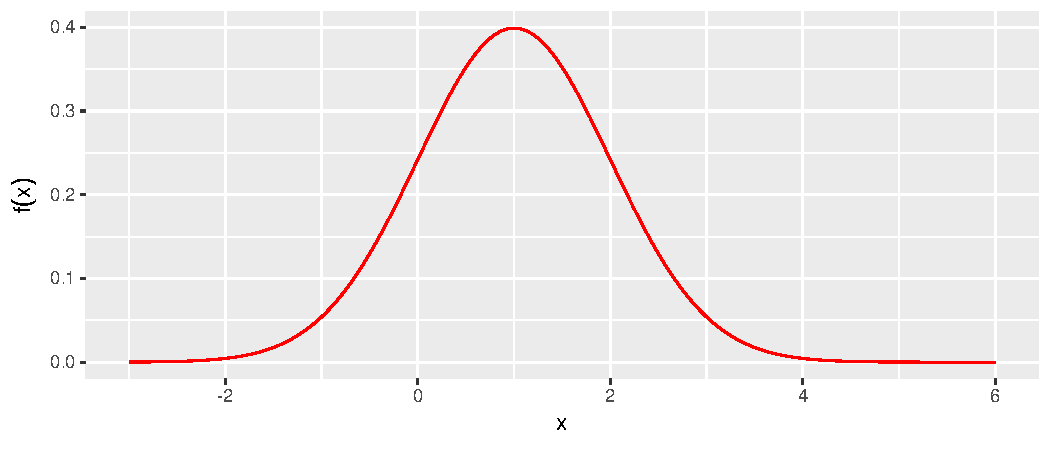
\includegraphics[width=\maxwidth]{figure/unnamed-chunk-3-1.pdf} 
\end{knitrout}

\onslide<2-|handout:1> 

\begin{knitrout}
\definecolor{shadecolor}{rgb}{0.969, 0.969, 0.969}\color{fgcolor}
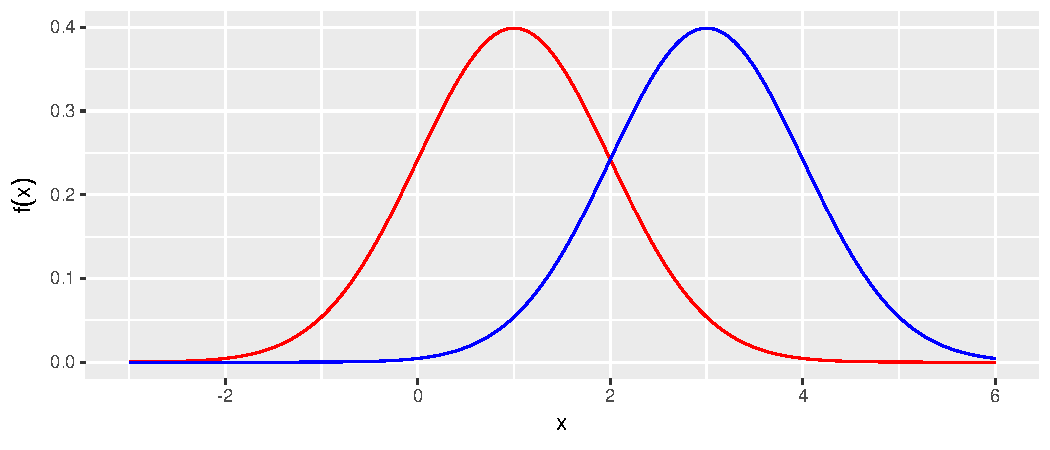
\includegraphics[width=\maxwidth]{figure/unnamed-chunk-4-1.pdf} 
\end{knitrout}

\end{overprint}
\begin{itemize}
\item \vspace{-0.4cm}
The \textcolor{red}{red} curve is the pdf of a $\rv$ $X$ with $\colorAonOne{\omE(X)=1},\colorBonTwo{\omV(X)=1}$.
\item The \textcolor{blue}{blue} curve is the pdf of the $\rv$ $W\omcoloneqq X+2$.
\end{itemize}
\begin{uncoverenv}<.->
\begin{alertenv}<.-.(2)>
\vspace{-0.1cm}
\begin{omx}
$\omE(W)=\AltQ{\omE(X+2)=\omE(X)+\omE(2)=\triggerOne 1+2=\omFinalAnswer 3.}$
\end{omx}
\end{alertenv}

\end{uncoverenv}

\begin{uncoverenv}<.->
\vspace{-0.35cm}
\begin{alertenv}<.-.(2)>
\begin{omx}
$\omV(W)=\AltQ{\omV(X+2)=\omV(X)=\triggerTwo{\omFinalAnswer 1}.}$
\end{omx}
\end{alertenv}

\end{uncoverenv}

\end{frame}
\begin{frame}{Visualizing $\omV(cX)=c^{2}\omV(X)$}

\begin{overprint}
\onslide<1|handout:0> 

\begin{knitrout}
\definecolor{shadecolor}{rgb}{0.969, 0.969, 0.969}\color{fgcolor}
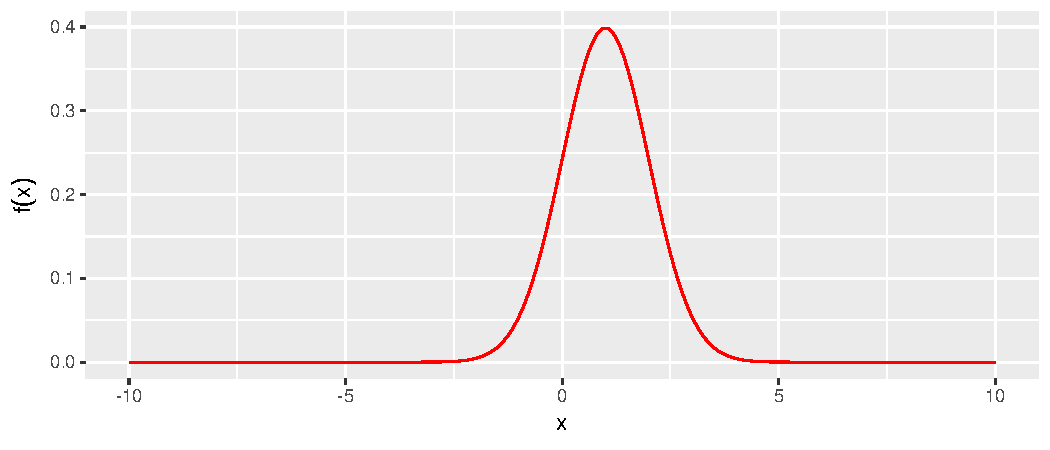
\includegraphics[width=\maxwidth]{figure/unnamed-chunk-5-1.pdf} 
\end{knitrout}

\onslide<2-|handout:1> 

\begin{knitrout}
\definecolor{shadecolor}{rgb}{0.969, 0.969, 0.969}\color{fgcolor}
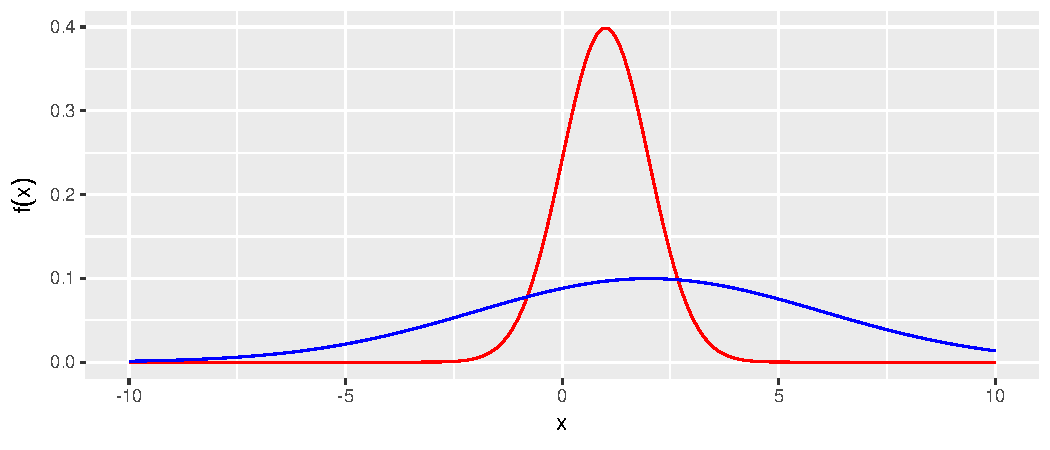
\includegraphics[width=\maxwidth]{figure/unnamed-chunk-6-1.pdf} 
\end{knitrout}

\end{overprint}
\begin{itemize}
\item \vspace{-0.4cm}
The \textcolor{red}{red} curve is the pdf of a $\rv$ $X$ with $\omE(X)=1,\omV(X)=1$.
\item The \textcolor{blue}{blue} curve is the pdf of the $\rv$ $W\coloneqq2X$.
\end{itemize}
\begin{alertenv}<.-.(2)>
\begin{uncoverenv}<.->
\vspace{-0.1cm}
\begin{omx}
$\omE(W)=\AltQ{\omE(2X)=2\cdot\omE(X)=2\cdot1=\omFinalAnswer 2.}$
\end{omx}
\end{uncoverenv}

\end{alertenv}

\begin{alertenv}<.-.(2)>
\vspace{-0.35cm}
\begin{uncoverenv}<.->
\begin{omx}
$\omV(W)=\AltQ{\omV(2X)=2^{2}\cdot\omV(X)=4\cdot1=\omFinalAnswer 4.}$
\end{omx}
\end{uncoverenv}

\end{alertenv}

\end{frame}

\begin{frame}{Income inequality}
\begin{itemize}
\item Suppose that variance of income in a country is our measure of income
inequality.
\item Suppose that Iran and Turkmenistan both discover huge amounts of new
oil reserves.
\item Iran decides to double everyone's income.
\item Turkmenistan decides to give $\currency{10\thousandsSeparator000}$
to every individual.
\end{itemize}
\begin{omx}
What happens to the measure of income inequality in Iran and, separately,
in Turkmenistan?
\end{omx}
\begin{itemize}
\item Let $X$ be income of an individual chose at random from Iran.
\item $\omV(2X)=2^{2}\omV(X)=4\omV(X)$, so \omFinalAnswer{inequality quadruples in Iran}.
\item Let $Y$ be the income of an individual chosen at random from Turkemnistan.
\item $\omV(Y+10\thousandsSeparator000)=\omV(Y)$, so \omFinalAnswer{inequality stays the same in Turkmenistan}.
\end{itemize}
\end{frame}

\subsubsection{Standard deviation}
\begin{frame}{Standard deviation}
\begin{block}{}
The standard deviation of $X$ is
\[
\omSD(X)\omcoloneqq\sqrt{\omV(X)}
\]
\end{block}
\begin{block}{}
Common notation is $\sigma_{X}\omcoloneqq\omSD(X)$.
\end{block}
\end{frame}
\begin{frame}{Reviewing new notation}
\begin{itemize}
\item $\mu_{X}\omcoloneqq\omE(X)$ and is pronounced ``mu x''.
\item $\sigma^{2}_{X}\omcoloneqq\omV(X)$ and is pronounced ``sigma squared
x'' or ``sigma x squared''.
\item $\sigma_{X}\omcoloneqq\omSD(X)$ and is pronounced ``sigma x''.
\end{itemize}
\end{frame}

\subsection{Back to a normal}
\begin{frame}{Notation}

\note<.>{Now that we are comfortable with mean and variance of random variables,
it's helpful to formally state the following:}
\begin{itemize}
\item Recall: the normal distribution has two \uline{parameters}, $\mu$
and $\sigma$:
\[
f(x)=\frac{1}{\sigma\sqrt{2\pi}}e^{-\frac{1}{2}\left(\frac{x-\mu}{\sigma}\right)^{2}}
\]
\item It is not a coincidence that we refer to the parameter $\mu$ as the
``mean'' and the parameter $\sigma$ as the ``standard deviation''.
\item That is, if $X$ is normally distributed, then the mean and variance
of $X$ completely determine the distribution.
\item We thus write $N(a,b^{2})$ to refer to a normal distribution with
mean $a$ and variance $b^{2}$ (i.e., standard deviation $b$).
\item $N(0,1)$ is called the \uline{\omemphA{standard} normal distribution}.\note<.>{although there an infinite amount of normal distributions, there's
only \emph{one} standard normal distribution.}
\end{itemize}
\begin{notation}
We use $\omeqcolor{\sim}$ to mean ``has the distribution''. e.g.,
$X\omeqcolor{\sim}N(0,1)$ means ``$X$ has the standard normal distribution.''
\end{notation}
\end{frame}
\begin{frame}[fragile]{Name that normal}

\begin{knitrout}
\definecolor{shadecolor}{rgb}{0.969, 0.969, 0.969}\color{fgcolor}
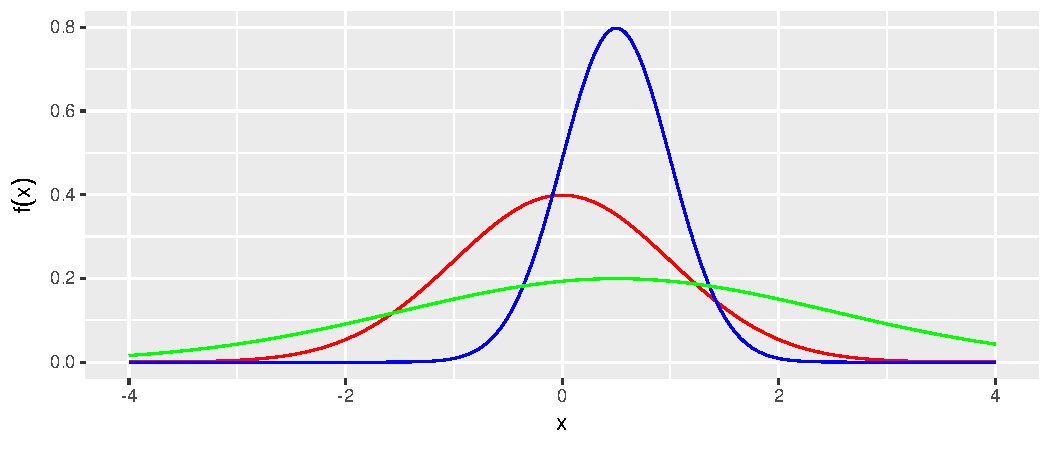
\includegraphics[width=\maxwidth]{figure/unnamed-chunk-7-1.pdf} 
\end{knitrout}

\begin{omx}
Densities of the following three distributions are shown above: $N(0,1)$,
$N(\frac{1}{2},\frac{1}{4})$, $N(\frac{1}{2},4)$. Which is which?
\end{omx}
\begin{block}{}
\answer{\textcolor{red}{$N(0,1)$} is the \textcolor{red}{red}, \action<\omalertA>{\textcolor{blue}{$N(\frac{1}{2},\frac{1}{4})$} is the \textcolor{blue}{blue},
and \textcolor{green}{$N(\frac{1}{2},4)$} is the \textcolor{green}{green}.}}
\end{block}
\end{frame}


\end{document}
